\section{Results}
In an exposure of 34~Kg per 224~days of liquid xenon a yield of 764 events are found in the region of interest,
which is compatible with the expectation of $756 \, \pm \, 5^{(stat.)} \, \pm 55^{(syst.)}$. The distribution 
of events from data are compared to the background expectation in Figure~\ref{fig:dataVSbkg} and with the relative
uncertainties.  
This result is interpreted via a binned profiled likelihood approach by means of the test statistic $\tilde{q}$
and its asymptotic distributions described in \cite{asympt}. 90\% CL$_s$ \cite{cls} confidence level limits are 
computed on the spin dependent cross section as a function of the WIMP mass and shown in Figure~\ref{fig:limits}.

\newpage
\begin{figure}[t!]
  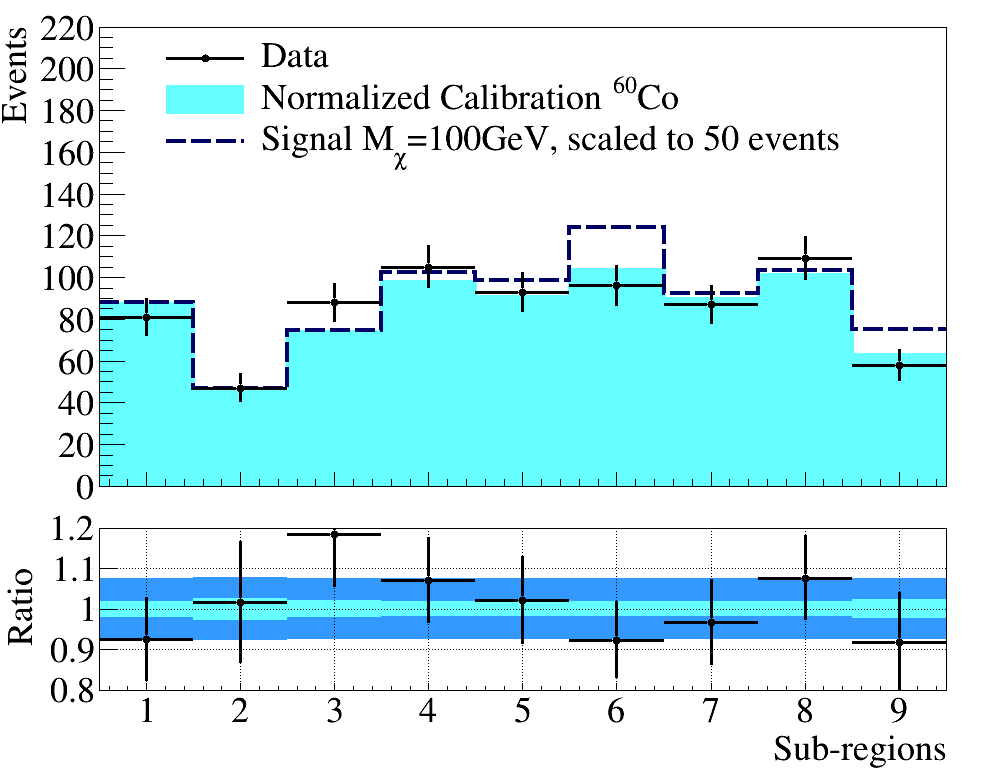
\includegraphics[width=\linewidth]{images/data_vs_bkg.png}
  \caption{Results, comparison between data and expected background.}
  \label{fig:dataVSbkg}
\end{figure}

\begin{figure}[h]
  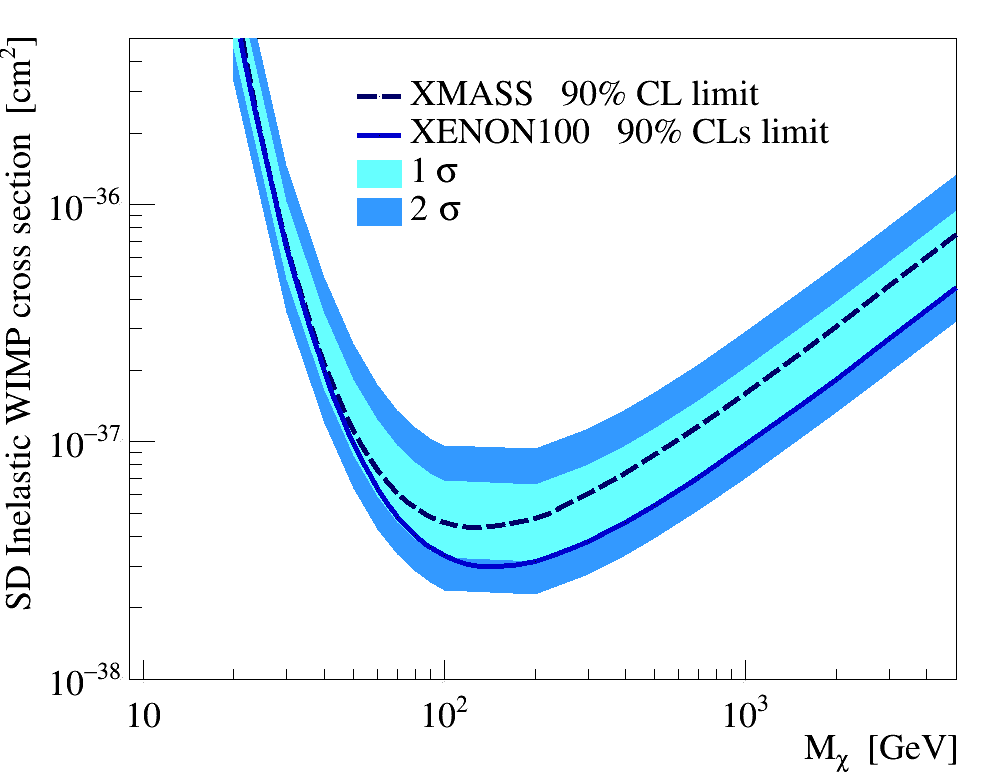
\includegraphics[width=\linewidth]{images/limit_reb.png}
  \caption{Observed and expected limits.}
  \label{fig:limits}
\end{figure}


\newpage
